\documentclass[conference]{IEEEtran}
\IEEEoverridecommandlockouts
% The preceding line is only needed to identify funding in the first footnote. If that is unneeded, please comment it out.
\usepackage{cite}
\usepackage{amsmath,amssymb,amsfonts,fullpage}
\usepackage{algorithmic}
\usepackage{graphicx}
\usepackage{textcomp}
\usepackage{xcolor}
\def\BibTeX{{\rm B\kern-.05em{\sc i\kern-.025em b}\kern-.08em
    T\kern-.1667em\lower.7ex\hbox{E}\kern-.125emX}}
\usepackage{fullpage,amsmath}
\usepackage{times}
\usepackage{xspace}

\usepackage{xspace}


\newcommand{\eat}[1]{}
\newcommand{\am}[1]{{\color{blue} \emph{[[AM: #1]]}}}
\newcommand{\arc}[1]{{\color{blue} \emph{[[ARC: #1]]}}}
\newcommand{\xh}[1]{{\color{purple} \emph{[[XH: #1]]}}}


\newcommand{\stitle}[1]{\vspace{.33em}\noindent\textbf{#1}~}

\newcommand{\system}{Crypt$\epsilon$\xspace}

\newcommand{\encD}{\boldsymbol{\tilde{\mathcal{D}}}}
\newcommand{\crossproduct}{\times}
\newcommand{\project}{\pi}
\newcommand{\filter}{\sigma}
\newcommand{\countagg}{count}
\newcommand{\groupbystar}{\gamma^{*,count}}
\newcommand{\groupby}{\gamma^{count}}
\newcommand{\countdistinct}{count^*}
\newcommand{\encT}{\boldsymbol{\tilde{T}}}
\newcommand{\encB}{\boldsymbol{B}}
\newcommand{\encC}{\boldsymbol{c}}
\newcommand{\encV}{\boldsymbol{V}}
\newcommand{\lap}{Lap}
\newcommand{\noisymax}{NoisyMax}
\newcommand{\postorder}{post}

\newcommand{\squishlist}{
	\begin{list}{$\bullet$}
		{
			\setlength{\itemsep}{0pt}
			\setlength{\parsep}{3pt}
			\setlength{\topsep}{3pt}
			\setlength{\partopsep}{0pt}
			\setlength{\leftmargin}{1.5em}
			\setlength{\labelwidth}{1em}
			\setlength{\labelsep}{0.5em} } }
	
\newcommand{\squishend}{
\end{list}  }


\title{Accurate Differentially Private Algorithms without a Trusted Data Collector}
\author{TBD}

\begin{document}
\maketitle

\begin{abstract}

\end{abstract}

\begin{IEEEkeywords}
Crypto-assisted Differential Privacy, Crypto Service Provider, 
\end{IEEEkeywords}

\section{Background}
\subsection{Notation}
\xh{Define notation for a databset $D$:the number of rows (users), the number of attributes (notations for attributes),...}

\subsection{Differential Privacy}
\begin{definition} An algorithm $\mu$
satisfies $\epsilon$-differential privacy ($\epsilon$-DP), where $\epsilon \geq 0$ is a privacy parameter, iff
 for any two datasets $D$ and $D'$ that differ in a single record, we have
\begin{gather}
\forall t \in Range(\mu), Pr \big[\mu(D) = t\big] \leq e^{\epsilon}Pr\big[\mu(D') = t\big]
\end{gather}
where $Range(\mu)$ denotes the set of all possible outputs
of the algorithm $\mu$.
\end{definition}

\xh{Need define sequential composition properties of DP here or at appendix.}

\begin{comment}\subsubsection{Local Differential Privacy}
\arc{Not final-placeholder}
In the local setting, there is no trusted third party. An aggregator
wants to gather information from users. Users
are willing to help the aggregator, but do not fully trust
the aggregator for privacy. For the sake of privacy, each
user perturbs her own data before sending it to the aggregator
(via a secure channel). 

Consider a setting where each user has a single value $v$, which can be viewed
as the user’s answer to a given question. The aggregator
aims to find out the frequencies of values among the
population. Such a data collection protocol consists of
the following algorithms:
\begin{enumerate}
\item Encode is executed by each user. The algorithm
takes an input value v and outputs an encoded value
x.
\item  Perturb, which takes an encoded value x and outputs
y. Each user with value v reports y =
Perturb(Encode(v)). For compactness, we use
PE(·) to denote the composition of the encoding
and perturbation algorithms, i.e., PE(·) =
Perturb(Encode(·)). PE(·) should satisfy $\epsilon$-local
differential privacy, as defined below.
\item Aggregate is executed by the aggregator; it takes all
the reported values, and outputs aggregated information.
\end{enumerate}
\begin{definition}
 Local Differential Privacy- An algorithm
$A$ satisfies $\epsilon$-local differential privacy ($\epsilon$-LDP),
where $\epsilon \leq 0$, if and only if for any input $v_1$ and $v_2$, we
have
\begin{gather} \forall y  \in Range(A) : Pr [A(v_1) = y] \leq e^{\epsilon} Pr [A(v_2) = y] \end{gather}
where $Range(A)$ denotes the set of all possible outputs
of the algorithm $A$.
\end{definition}
This notion is related to randomized response [24],
which is a decades-old technique in social science to collect
statistical information about embarrassing or illegal
behavior. To report a single bit by random response, one
reports the true value with probability p and the flip of the
true value with probability 1-p. This satisfies
(
ln p
1-p
)
-
LDP.
Comparing to the setting that requires a trusted data
curator, the local setting offers a stronger level of protection,
because the aggregator sees only perturbed data.
Even if the aggregator is malicious and colludes with all
other participants, one individual’s private data is still
protected according to the guarantee of LDP.
\subsubsection{Computational Differential Privacy}
\begin{definition}
 (IND-CDP privacy) An ensemble $\{f_\kappa\}\kappa  \in N$ of randomized
functions $f_\kappa : D \rightarrow R_\kappa$ provides $(\epsilon,
\kappa)$-ind-cdp if there exists a negligible function $negl(\cdot)$ such that for every nonuniform p.p.t turing machine (“distinguisher”) $A$, every polynomial $p(\cdot)$, every sufficiently large $\kappa \in N$ all
data sets $D,D' \in \mathcal{D}$ of size at most $p(\kappa)$ such that $|D-D'|\leq  1$, and
every advice string $z_{\kappa}$ of size at most $p(\kappa)$, it holds that \begin{gather}
Pr [A_{\kappa}(f_{\kappa}(D)) = 1] \leq e^{\epsilon} \times Pr[A_{\kappa}(f_{\kappa}(D')) = 1]
+ negl(\kappa)\end{gather}
where we write $A_\kappa(x)$ for $A(1^{\kappa}, z_{\kappa}, x)$ and the probability is taken over
the randomness of mechanism $f_\kappa$ and adversary $A_\kappa$.
\end{definition}
\end{comment}


\subsection{Cryptographic Primitives}
\stitle{Linearly Homomorphic Encryption (\textsf{LHE}).}
Let $(\mathcal{M}, +)$ be a finite group. A \textsf{LHE} scheme
for messages in $\mathcal{M}$ is defined as three steps:
(i) The key generation algorithm $Gen(\cdot)$ takes the security parameter $\kappa$ as input and outputs
a pair of secret and public keys, $(s_k, p_k) \leftarrow Gen(\kappa)$;
(ii) The encryption algorithm $Enc(\cdot)$ which is a randomized algorithm encrypts a message $m \in \mathcal{M}$ via the public key $p_k$, to generate ciphertext $c \leftarrow Enc_{pk}(m)$;
(iii) The decryption algorithm $Dec(\cdot)$ is a deterministic function that uses the secret key $s_k$ to recover the original plaintext from a ciphertext $c$.
\eat{
\begin{itemize}
\item Key Generation ($Gen$) -The key generation algorithm $Gen$ takes the security parameter $\kappa$ as input and outputs
a pair of secret and public keys, $(s_k, p_k) \leftarrow Gen(\kappa)$.
\item Encryption ($Enc$) - This is a randomized algorithm that encrypts a message $m \in \mathcal{M}$ via the public key $p_k$, to generate ciphertext $c \leftarrow Enc_{pk}(m)$.
\item Decryption ($Dec$) - The decryption algorithm $Dec$ is a deterministic function that uses the secret key $s_k$ to
recover the original plaintext from a ciphertext c.
\end{itemize}
}

In addition, linearly homomorphic encryption scheme supports the two operations $\oplus$ and $\otimes$ with the following properties:
\begin{eqnarray}
Dec_{sk}(Enc_{pk}(m_1)\oplus\cdots Enc_{pk}(m_i)) = m_1+\cdots+m_i \\
Dec_{sk}(Enc_{pk}(m,i)) = m \cdot i
\end{eqnarray}
where $m\in \mathcal{M}$ and $i\in \mathbb{Z}^+$.

\xh{(1) check if this rewrite above is correct. (2) simplify the remaining paragraphs as LHE. (3) Most importantly, we need state what `security guarantee' does these encryption scheme provides.}

\eat{
\begin{itemize}\item Operator $\oplus$ - Let $c_1 \leftarrow Enc_{pk}(m1), \ldots, c_a \leftarrow Enc_{pk}(m_a), a \in \mathcal{Z}_{>0}$. Then we have  $Pr\big[Dec_{sk}(c_1\oplus c_2 ...\oplus c_a)=    m_1 + \ldots   + m_a\big]=1$  
\item Operator $cMult(a,c)$ - Let $c\leftarrow  Enc_{sk}(m)$. Then  \\ $Dec_{sk}\big(cMult(a,c)\big)=am$ where $cMult(a,c)=c\oplus \ldots \oplus c$ (a times) \end{itemize}
}

\stitle{Labeled Homomorphic Encryption(\textsf{labHE}).}
Let $(Gen,Enc,Dec)$ be an \textsf{LHE} scheme with security parameter $\kappa$ and message space $\mathcal{M}$. Assume that a multiplication operation is given in $\mathcal{M}$, i.e., is a finite ring. Let also $\mathcal{F}:\{0,1\}^s \times \mathcal{L}\rightarrow \mathcal{M}$ be a pseudo-random function with speed space $\{0,1\}^s$( s= poly($\kappa $)) and the label space $\mathcal{L}$. Define
\begin{itemize}
\item $labGen(\kappa)$ - On input $\kappa$, it runs $Gen(\kappa)$ and outputs $(sk,pk)$
\item $localGen(pk)$ -  For each user $i$ and with the public key as input, it samples a random seed $\sigma_i \in \{0,1\}^s$ and computes $pk_i = Enc_{pk}(\ddot{\sigma_i})$ where $\ddot{\sigma_i}$ is an  encoding of $\sigma_i$ as an  element of $\mathcal{M}$. It outputs $(\sigma_i,pk_i)$.
\item $labEnc_{pk}(\sigma_i, m , \tau)$: On input a message $m \in \mathcal{M} $ with label $\tau \in \mathcal{L}$  from user $i$, it computes $b=\mathcal{F}(\sigma_i, \tau))$ and outputs the labeled ciphertext $\mathbf{c}=(a,c) \in \mathcal{M} \times \mathcal{C}$ with $ a= m- b$ in $\mathcal{M}$ and $c=Enc_{pk}(b)$.
\item $labDec_{sk}(\mathbf{c})$ - This functions inputs a cipher $\mathbf{c}=(a,c) \in \mathcal{M} \times \mathcal{C}$ encrypted under the labHE scheme and decrypts it as $m=a-Dec_{sk}(c)$.
\end{itemize}
In addition to the aforementioned operations supported by a \textsf{LHE}  scheme, \textsf{labHE} supports multiplication of two labeled ciphers as follows.
\begin{itemize}\item $labMult(\mathbf{c}_1,\mathbf{c}_2)$ -
On input two labeled ciphers $\mathbf{c}_1=(a_1,c_1)$ and $\mathbf{c}_2=(a_2,c_2)$, it computes a "multiplication" ciphertext $\mathbf{d}=labMult(\mathbf{c_1,c_2})=Enc_{pk}(a_1,a_2)\odot cMult(c_1,a_2) \odot cMult(c_2,a_1)$. Observe that $Dec_{sk}(\mathbf{d})=m_1\cdot m_2 -b_1 \cdot b_2$.
\item $labMultDec_{sk}(c_1,c_2,\mathbf{d})$ - On input two labels $c_1,c_2$ of two labHE ciphers $\mathbf{c_1},\mathbf{c_2}$ and the output $\mathbf{d}$ of $labMult(\mathbf{c_1},\mathbf{c_2})$, it decrypts the product as $m_3=Dec_{sk}(\mathbf{d})+Dec_{sk}(c_1)\cdot Dec_{sk}(c_2) = m_1\cdot m_2$ .    \end{itemize}
In this paper we propose an efficient way of extending the $labMult$ operation for a $n$-way multiplication in section \ref{implementation}.


\stitle{Secure Computation.}
%\arc{Not final:placeholder}
Garbled circuit, also known as Yao's protocol \cite{Yao,yao2},  is a generic method for secure multi-party computation. In this paper we just discuss the two-party scenario but it can be generalized to $n > 2$ parties. In its basic form, a garbled circuit allows two-party evaluation of a function $f(x_1,x_2)$ in the presence of semi-honest adversaries. The protocol is run between two data owners with respective private inputs $x_1$ and $x_2$ such that at the end, no party learns more  
than what is revealed from the output value $f(x_1,x_2)$. In the protocol, one of the parties called
generator, builds a "garbled" version of a circuit computing $f$ and sends it over to the second party, called evaluator, alongside the garbled input values 
corresponding to $x_1$.  Upon receiving the circuit, the evaluator 
engages in an oblivious transfer protocol with the generator to obliviously obtain the garbled input for $x_2$. Finally the evaluator can securely compute the  output $f(x_1, x_2)$ from the garbled circuit and the corresponding garbled inputs for $\{x_1,x_2\}$.

\begin{comment}\subsection{Data \& Queries}
\subsubsection{One-hot-encoding} - One-hot-coding is a way of representation for categorical attributes. First the data is converted to an integral representation as follows. Let us assume that the total number of categories is $k$ then each category is represented by an unique integer in $\{1,..., k\}$. Now the one-hot-encoding for a category $x$ with integral representation $t , t \in [k]$ is given by a $k$-lengthed vector $\tilde{x}$ such that $tilde{x}[t]=1, \forall i \in [k], i\neq t, \tilde{x}[i]=0$. 
For example consider an attribute $Age$ with domain $\{1,...,100\}$. In this case since the categories itself are integral, we can skip the first step. Thus the one-hot-encoding corresponding to a value $x=30, type(x)=Age$ is given by $\tilde{x}[30]=1, $equivalent to. In fact the one-hot-coding can be generalized to  represent data across $n$ different attributes. For example, in addition to the aforementioned $Age$ attribute consider  another attribute  $Gender$ with domain $\{Male, Female, Other\}$. Let the categorical values $\textit{Male, Female }$ and $Other$ be represented by integers $1, 2$ and $3$ respectively. Thus a one-hot-encoding for a value $X=<1,30> \in Age \times Gender$ is given by \begin{gather*}i \in [300] \\\tilde{X}[i]=\begin{cases}1, \textit{ if } i =30,\\ 0 , \textit{ otherwise }\end{cases}\end{gather*}
\begin{comment}\subsubsection{Unary Query Type}
We support unary queries that is queries that operate on a single dataset
\am{Single Table, categorical attributes, in tabular form (and not in vector form), Counting queries ...}
Let condition formula, $\phi$ be a Boolean
condition that can be evaluated on any tuple of $D$ and let $\phi(D )$ 
denote the number of tuples in $D$ for which $\phi$ is true. A number of
operators in Crypt$\epsilon$ answer linear queries over the table. A linear
query is the linear combination of any finite set of condition counts:
\begin{definition}
 (Linear counting query (declarative)). A linear query
$q$ on $D$ is defined by conditions $\phi_1 \ldots \phi_k$ and coefficients $c_1 \ldots c_k \in \mathcal{Z}$
 and returns \begin{equation}q(D ) = c_1\phi_1(D) + \ldots + c_k\phi_k (D ) \label{countingq}\end{equation}
\end{definition}
\end{comment}

\section{Protocols}
\subsection{Notations:} $A$ - Represents an attribute\\$dom(A)$ - Domain of attribute  $A$\\$s_A$ - Size of the dom($A$)\\$v_i, i \in [s_A]$-$dom(A)=\{v_1,v_2,\ldots, v_{s_A}\}$\\$ct_{A,i}$-\# records with value $v_i$ for attribute $A$\\m-\# number of data onwers\\$\mathcal{D}$- Encrypted database\\ $\mathcal{A}=\{\mathcal{A}_1,...\mathcal{A}_l\}$ - The set of attributes in the relational schema of $\mathcal{D}$\\
$x \times y$ table $T$ - A table  with $x$ rows/records and $y$ columns one for each  attribute, serves as one of the inputs to a transformation primitive
\\
$x' \times y'$ table $T'$ - A table  with $x'$ rows/records and $y'$ columns one for each  attribute, serves as the output of a transformation primitive\\
$\mathcal{E}(x)$- Represents the one-hot-coding for x\\
Boldface characterizes encrypted value\\
$\tilde{}$ characterizes that the data is in one-hot-coding\\
Throughout this section we will assume that there is an encryption
scheme $\mathcal{E}$ is a $4$-tuple $(Gen,Enc,Dec,Eval)$, which is
homomorphic with respect to all functions in a set $\mathcal{F}$.

\subsection{Parties}

There are three type of entities involved in the protocol: {\it
  analytics server (AS)}, {\it crypto-service provider (CSP)}, and
users. CSP runs the key-generation algorithm $Gen(\lambda)$ and 
obtains a pair of keys $(sk,pk)$. We assume that a secure mechanism 
is used to distribute $pk$ to  AS and the users. 

\subsection{Protocol 1 (Uses Homomorphic Encryption)}

\noindent
{\bf Step 1:} We assume that $U=\{ u_1, \cdots, u_n \}$ is the set of
users. Whenever a user $u_i$ needs to send a value $v$ to AS, he/she
sends the encrypted value $Enc_{pk} (v)$ to AS.

\noindent
{\bf Step 2:} Assume that AS has encryptions of some values
(i.e. $Enc_{pk}(v_1),\cdots,Enc_{pk}(v_m)$). AS generates a random
value $r$ according to some distribution (e.g. a random value
corresponding to the Laplace or Guassian distribution) and needs to
compute some function $G(f(v_1,\cdots,v_m),r)$ (we can think of $G$ as
DP version of the function $f$). For example, if we are computing the
sum of the values in a differentially private manner then
$f(v_1,\cdots,v_m) = \sum_{i=1}^m v_i$, $r$ is distributed according
to the Laplace distribution, and $G(x,y) = x+y$. Now assume that the
function $G(f(v_1,\cdots,v_m),r) \in \mathcal{F}$. Assuming that for
$1 \leq i \leq m$, $c_i = Enc_{pk}(v_i)$, AS computes
$Eval(G,c_1,\cdots,c_m,r)$ which yields $Enc_{pk}(G(f(m_1,\cdots,m_r),r))$.

\noindent
{\bf Step 3:} AS generates another random value $z$ (assuming that
addition is in the set of functions $\mathcal{F}$) and computes
$Enc_{pk}(G(f(m_1,\cdots,m_r),r)+z)$ and sends it to CSP. CSP decrypts
the value using the secret $sk$ and obtains $G(f(m_1,\cdots,m_r),r)+z$
and sends it to AS.  AS subtracts $z$ and obtains
$G(f(m_1,\cdots,m_r),r)$, which is the desired result.

\subsection{Protocol 2 (Uses SMC)}

If $G(f(v_1,\cdots,v_m),r) \not\in \mathcal{F}$, then we cannot simply
use homomorphic encryption and thus we use secure multiparty
computation (SMC).

{\it Inputs:} AS's input $i$ to the SMC protocol is
$Enc_{pk}(v_1),\cdots,Enc_{pk}(v_m)$ and a random variable $r$. CSP's
input $j$ is the secret key $sk$. The function $z (i,j)$ corresponds
to the following two steps:
\begin{itemize}
\item Decrypt $Enc_{pk}(v_1),\cdots,Enc_{pk}(v_m)$ using $sk$ and obtain
$v_1,\cdots,v_m$.
\item Compute $G(f(v_1,\cdots,v_m),r)$
\end{itemize}

{\it Output:} At the end of the protocol, AS receives the output of the
function $z(i,j)$ and CSP receives no output.

\am{Does the CSP get to see the plaintext of the original entries $v_1, \ldots, v_m$?}



%!TEX root = main.tex

\section{\system Primitives}\label{sec:primitives}

Given a database schema $\langle A_1,\ldots,A_k \rangle$ and an encrypted instance of this database, $\encD$, \system permits data analysts to author \textit{logical} \system programs on $\encD$ with differential privacy guarantee.  The logical programs mainly consist of data transformation operators inspired by relational algebra and differentially private measurement operators. These programs can  have constructs like looping and conditionals, and can arbitrarily post-process outputs of measurement operators. \system compiles these logical programs into \system protocols that can work on the encrypted data on the \textsf{AS} and \textsf{CSP}. Though these logical \system programs are designed to run on encrypted data, when operating them on plaintext data, they give differential privacy under \textsf{CDP}.
%\am{Should we say that logical \system program when operating on the raw data gives you DP under CDP? }

In this section, we define the primitives for data transformations and differentially private measures (summarized in Table~\ref{tab:primitives}). Then, we illustrate how to write logical programs using these primitives to express state-of-the art DP algorithms under the \cdp model. In Section~\ref{sec:implementation} we describe how \system compiles these down to protocols that work on encrypted data.

% Please add the following required packages to your document preamble:
% \usepackage{multirow}


\begin{table*}[]
\small{
\caption {\system Primitives}\label{tab:primitives}
\begin{tabular}{|l|l|l|l|l|l|}
\hline
\bf{Types}                           & \bf{Name}         & \bf{Notation} & \bf{Input} & \bf{Output} & \bf{Functionality} \\ \hline \hline
\multirow{7}{*}{Transformation} & \multirow{2}{*}{\textsf{CrossProduct}} &  \multirow{2}{*}{$\crossproduct_{A_i,A_j\rightarrow A'}(\cdot)$} & 

\multirow{2}{*}{$\encT$}   &  \multirow{2}{*}{$\encT'$}   & Generates a new attribute  $A'$ (in one-hot-coding) to represent\\ & & & & & the data for both the attributes $A_i$ and $A_j$   \\ \cline{2-6}
                                & \textsf{Project}     & $\project_{A^*}(\cdot)$  &  $\encT$       &  $\encT'$       &  Discards all attributes but $A*$ \\ \cline{2-6}
                                & \textsf{Filter}       & $\filter_{\phi}(\cdot)$   &  $\encT$      &   $\encB'$     &  Zeros out records not satisfying $\phi$    in $\encB$          \\ \cline{2-6}
                                & \textsf{Count}             & $\countagg(\cdot)$         & $\encT$  &  $\encC$    &  Counts the number of 1s in $\encB$               \\ \cline{2-6}
                                & \textsf{GroupByCount*}             & $\groupbystar_{A}(\cdot)$ &  $\encT$  & $\encV$    & Returns encrypted histogram of $A$                \\ \cline{2-6}
                                & \textsf{GroupByCount}              & $\groupbystar_{A}(\cdot)$    &$\encT$       & $\tilde{\encV}$        &  Returns encrypted histogram of $A$ in one-hot-encoding    \\ \cline{2-6}
                                & \textsf{CountDistinct}             & $\countdistinct(\cdot)$     &    $\encV$   & $\encC$   &  Counts the number of non-zero values in $\encV$       \\ \hline
\multirow{2}{*}{Measurement}    & \textsf{Laplace}     & $\lap_{\epsilon,\Delta}(\cdot)$    &  $\encV$      &   $\hat{V}$    &  Adds Laplace noise to $\encV$    \\ \cline{2-6}
                                & \textsf{NoisyMax}     & $\noisymax_{\epsilon,\Delta}^k(\cdot)$         & $\encV$       &  $\hat{\mathcal{P}}$      &  %Adds Laplace noise to $\encV$ and 
                                Returns indices of the top $k$ noisy values              \\ \hline
\end{tabular}
}
\end{table*}


\eat{
\begin{table*}[h!]
\small
\caption {\system Primitives}
 \begin{tabular}{@{}l c@{}c@{}l@{}}  \toprule
\multicolumn{1}{c}{\textbf{Primitives}} & \textbf{Input}  & \textbf{Output}  & \multicolumn{1}{c}{\textbf{Functionality}}  \\ [0.5ex] 
 \midrule \midrule \textsf{CrossProduct} &$\tilde{\mathbf{T}}, A_i, A_j$ & $\tilde{\mathbf{T'}}$ & Generates  one-hot-coding for the\\&& & attribute $A_i\times A_j$ 
 \\\textsf{Project}&$\tilde{\mathbf{T}}, A^*$&$\tilde{\mathbf{T'}}$ &Discards all attributes but $A^*$
 \\\textsf{Filter}&$\tilde{\mathbf{T}},\phi$&$\tilde{\mathbf{B}}$&Zeros out records not satisfying $\phi$
 \\\textsf{Count}&$\tilde{\mathbf{T}}$&$\mathbf{C}$&Counts the number of records in $\textbf{B}$ 
 \\$\textsf{GroupBy}^*$ &$\tilde{\mathbf{T}},A$&$\mathbf{V}$& Returns encrypted histogram of $A$
 \\\textsf{GroupBy} &$\tilde{\mathbf{T}},A$ &$\tilde{\mathbf{V}}$ &Returns encrypted histogram of $A$\\&&& in one-hot-coding
 \\\textsf{CountDistinct} &$\mathbf{V}$&$\mathbf{C}$ &Counts the number of non-zero values in $\textbf{V}$
 \\\textsf{Laplace}&$\textbf{V},\epsilon$ &$\hat{\textbf{V}}$ & Both \textsf{CSP} and {AS} adds Laplace noise to $\textbf{V}$ 
 \\\textsf{NoisyMax} & $\textbf{V},\epsilon, k$&$P$ &Outputs top k values from noisy vector $\textbf{V}$\\
  [1ex] 
 \bottomrule
 \end{tabular}
\end{table*}
}


\subsection{Transformation Primitives}\label{sec:transformation_primitives}
Transformation primitives take an encrypted data as input and output a transformed encrypted data.  These primitives thus work completely on the encrypted data and do not expend any privacy budget. Three types of data are considered in this context: (1) an encrypted table of $x$ rows and $y$ columns/attributes, denoted by $\encT$, where each attribute value is represented by encrypted one-hot-encoding of the value; (2) an encrypted vector of numbers, denoted by $\encV$; and (3) an encrypted scalar, denoted by $\encC$. In addition, every encrypted table $\encT$ of $x$ rows has a encrypted bit vector $\encB$ of size $x$ to indicate whether the record is relevant to the program at hand. If the $i$-th bit value of $B$ is $1$, then the $i$-th row in $\encT$ will be used for answering the current program and vice versa. The input to the very first transformation primitive in \system program is the encrypted database $\encD$ with all bits of $\encB$ set to be $1$. For brevity, we just use $\encT$ to represent both the encrypted table $\encT$ and $\encB$. The transformation primitives are detailed below.

\stitle{{\normalfont(1)} \textsf{CrossProduct}} $\crossproduct_{(A_i,A_j)\rightarrow A'}(\encT)$: This primitive transforms the two encrypted one-hot-encodings for attributes $A_i$ and $A_j$ in $\encT$ into a single encrypted one-hot-encoding of a new attribute $A'$. The domain of the new attribute $A'$ is the cross product of the domains for $A_i$ and $A_j$. The resulting table $\encT'$ has one column less than $\encT$. Thus, the construction of the one-hot-coding of the entire $y$-dimensional domain can be computed by repeated application of this primitive. 	
%1) \textbf{\textsf{CrossProduct}}:$\crossproduct_{A_1,A_2}(\tilde{\mathbf{T}})$ - Given encrypted one-hot-codings for two different attributes $A_1$ and $A_2$ of domain sizes $s_{A_1}$ and $s_{A_2}$ respectively, the goal of this transformation is to compute the encrypted one-hot-coding for the entire two-dimension domain of the new $\lq$attribute' $A_1\times A_2$ of size $s_{A_1}\cdot s_{A_2}$. Thus this transformation takes as input a $x \times y $ table, $\tilde{\mathbf{T}}$ defined over attribute set $A=\{A_1,A_2,...,A_y\}$ where each cell $\tilde{\mathbf{T}}[i,j] , i \in [x], j \in [y], 2 \leq y \leq k$ corresponds to the encrypted one-hot-coding for attribute $A_j$ for the data owner $\textsf{DO}_i$ and outputs a $x \times (y-1)$ table with attribute set $\{A_1\times A_2,A_3,\ldots,A_{y}\}$.  Note that the construction of the one-hot-coding of the full $y$-dimension domain can be computed by repeated application of this transform. 	

\stitle{{\normalfont(2)} \textsf{Project}} $\project_{\bar{A}}(\encT)$: This primitive projects $\encT$ on  a subset of attributes $\bar{A}$ of the input table. All the attributes that are not in $\bar{A}$ are discarded from the output table $\encT'$.
	%2) \textbf{\textsf{Project}} : $\project_{A^*}(\tilde{\mathbf{T}})$- In addition to the $ x \times y$ table, $\tilde{\mathbf{T}}$ over attribute set $\{A_1, A_2, ..., A_y\}$, the \textsf{Project} transformation takes a set of attributes $A*=\{A^*_1,...A^*_p\}, p < y$ as inputs. The result of the transformation is defined as the $x \times p$ data source table where each record is just restricted to the attribute set $A^*$, i.e., it discards all other attributes. 
	%Infact it is analogous to the operation of marginalization which is described as follows.
	%Assuming  $A$ and $B$ to be two attributes with finite domains, let $x$ be a vector of counts representing a histogram over the cross product of the domain (with $|A|*|B|$ entries).
	%Marginalization over the attribute $B$ results in a vector of counts on the attribute $A$ alone by adding up counts corresponding to the same value of $A$.  


\stitle{{\normalfont(3)} \textsf{Filter}} $\filter_{\phi}(\encT)$: This primitive specifies a filtering condition, represented by a boolean predicate $\phi$ defined over a subset of attributes $\bar{A}$ of the input table $\encT$. The predicate can be expressed as a conjunction of range conditions over $\bar{A}$, i.e. for a row $r \in [x]$ in $\encT$, $\phi(r) = \bigwedge_{A_i \in \bar{A}} ~~(r.{A_i} \in V_{A_i})$,  where $r.A_i$ is value of attribute $A_i$ in row $r$ and $V_A$ is a subset of values (can be a singleton too) that attribute $A_i$ can take.  For example, $Age\in [30,40]\wedge Gender=M$ can be one such  filtering condition. The \textsf{Filter} primitive affects only the associated encrypted bit vector of $\encT$ and keeps the actual table untouched.  In this primitive, if any row $r \in [x]$ in $\encT$ does not satisfy the filtering condition $\phi$, the corresponding $r^{th}$ bit in $\encB$ will be set to $labEnc_{pk}(0)$; otherwise, the corresponding bit value in $\encB$ is kept unchanged.  Thus the \textsf{Filter} transformation suppresses all the records that are extraneous to answering the program at hand (i.e., does not satisfy $\phi$) by explicitly zeroing the corresponding indicator bits and outputs the table $\encT'$ with the updated indicator vector.


\stitle{{\normalfont(4)} \textsf{Count}} $\countagg(\encT)$: This primitive simply counts the number of rows in $\encT$ that are pertinent to the program at hand, i.e. the number of $1$s in its associated bit vector $\encB$.  This primitive outputs an encrypted scalar $\encC$. 
%Typically, this transformation is followed by a measurement primitive and is immediately preceded by a \textsf{Filter} primitive. \\
% 4) \textbf{\textsf{Count}}$:\countagg(\mathbf{T})$  - The \textsf{Count} transformation outputs the encrypted value of the non-noisy true count for the program at hand. For answering linear counting queries, typically \textsf{Count}  is the last transformation to be applied and is immediately preceded by a \textsf{Filter} transformation. Recall that the \textsf{Filter} transformation sets bit $i \in [m]$ to be 1 (encrypted) if the $i^{th}$ record satisfies the filter condition and 0 otherwise and outputs this encrypted $m\times 1$ vector. Hence the \textsf{Count} primitive simply adds up all the entries of this bit vector $\mathbf{B}$ and  outputs the sum which is a single encrypted value. 

\stitle{{\normalfont(5)} \textsf{GroupByCount*}} $\groupbystar_{A}(\mathbf{\tilde{T}})$: The  \textsf{GroupByCount*} primitive buckets the input table $\mathbf{\tilde{T}}$ into groups of records having the same value for an attribute $A$. The output of this transformation is thus, an encrypted  vector $\mathbf{V}$ which is the encrypted histogram for $A$.    This primitive serves as a preceding transformation for other Crypt$\epsilon$ primitives such as \textsf{NoisyMax}, \textsf{CountDistinct}.

\stitle{{\normalfont(6)} \textsf{GroupByCount}} $\groupby_{A}(\mathbf{\tilde{T}})$ : This primitive is similar to the aforementioned \textsf{GroupByCount*} primitive. The only difference between the two is that, \textsf{GroupByCount} outputs the encrypted histogram of attribute $A$ with each count represented in one-hot-coding, $\tilde{V}$.  This transformation allows us to answer queries based on the count of a particular value for attribute $A$.

\stitle{{\normalfont(7)} \textsf{CountDistinct } }$\countdistinct(\mathbf{V})$: As mentioned above, this primitive is always preceded by a \textsf{GroupByCount*} primitive. Hence the input vector $\mathbf{V}$ is an encrypted histogram for some attribute $A$ and this primitive returns the number of distinct values of $A$ that appear in  $\boldsymbol{\tilde{\mathcal{D}}}$ by counting the non-zero entries of $V$.
%The input to Crypt$\epsilon$ is an encrypted instance of a database $\boldsymbol{\tilde{\mathcal{D}}}$ with a single relational schema $\langle \mathcal{A}_1,\mathcal{A}_2, . . . ,\mathcal{A}_l\rangle$. Each attribute $\mathcal{A}_i$ is assumed to be discrete (or suitably discretized) and represented in one-hot-coding form.



\eat{
Transformation primitives take as input an encrypted source variable (a table of size $x \times y, x,y \in \mathcal{Z}_{\geq 0}$) and output a transformed data source (again  a table $x' \times y', x',y' \in \mathcal{Z}_{\geq 0}$) that is still encrypted. Typically $x$ and $x'$ are equal to $m$, the total number of data owners, i.e., every tuple in the data source tables corresponds to the record of a single data owner. In case $x=1$ or $x'=1$ the data source is an encrypted vector and we represent it as $\mathbf{V}$.
The transformation primitives are mostly carried out by the \textsf{AS} on its own; this is enabled by our use of labeled homomorphic encryption scheme which allows us to perform certain operations, specifically multiplication and addition, directly over the encrypted data. %Only two transformations  (\textsf{GroupBy} and \textsf{CountDistinct}) need to be computed via a secure computation protocol between the \textsf{AS} and the \textsf{CSP}. 
Since these primitives work entirely on encrypted data, they do not expend the privacy budget. However these operators can affect the privacy analysis through their stability. Every transformation in Crypt$\epsilon$ has a well-established stability.
For each record of the database $\boldsymbol{\tilde{\mathcal{D}}}$ (i.e., data corresponding to a single data owner) we maintain an encrypted bit which indicates whether the record is relevant to the program at hand. Let $\mathbf{B}$ represent this bit vector where $\mathbf{B}[i]$ corresponds to this indicator bit for the $i^{th}$ record.  If $\mathbf{B}[i] =Enc_{pk}(1)$, then the $i^{th}$ record is to be considered for answering the current program and vice versa. Only one of the transformation, \textsf{Filter} alters the bit vector $\mathbf{B}$. Before every program execution, $\mathbf{B}$ is initialized to a 1-vector. 
\begin{enumerate}

	\item \textsf{CrossProduct} ($\tilde{\mathbf{T}}, A_i, A_j$) - Given encrypted one-hot-codings for two different attributes $A_1$ and $A_2$ of domain sizes $s_{A_1}$ and $s_{A_2}$ respectively, the goal of this transformation is to compute the encrypted one-hot-coding for the entire two-dimension domain of the new $\lq$attribute' $A_1\times A_2$ of size $s_{A_1}\cdot s_{A_2}$. Thus this transformation takes as input a $x \times y $ table, $\tilde{\mathbf{T}}$ defined over attribute set $A=\{A_1,A_2,...,A_y\}$ where each cell $\tilde{\mathbf{T}}[i,j] , i \in [x], j \in [y], 2 \leq y \leq k$ corresponds to the encrypted one-hot-coding for attribute $A_j$ for the data owner $\textsf{DO}_i$ and outputs a $x \times (y-1)$ table with attribute set $\{A_1\times A_2,A_3,\ldots,A_{y}\}$.  Note that the construction of the one-hot-coding of the full $y$-dimension domain can be computed by repeated application of this transform. 	
    
	
	\item \textsf{Project}($\tilde{\mathbf{T}},A^*$)- In addition to the $ x \times y$ table, $\tilde{\mathbf{T}}$ over attribute set $\{A_1, A_2, ..., A_y\}$, the \textsf{Project} transformation takes a set of attributes $A*=\{A^*_1,...A^*_p\}, p < y$ as inputs. The result of the transformation is defined as the $x \times p$ data source table where each record is just restricted to the attribute set $A^*$, i.e., it discards all other attributes. \\
	%Infact it is analogous to the operation of marginalization which is described as follows.
	%Assuming  $A$ and $B$ to be two attributes with finite domains, let $x$ be a vector of counts representing a histogram over the cross product of the domain (with $|A|*|B|$ entries).
	%Marginalization over the attribute $B$ results in a vector of counts on the attribute $A$ alone by adding up counts corresponding to the same value of $A$.  
  \item \textsf{Filter}($\tilde{\mathbf{T}},\phi$) - Let $\tilde{\mathbf{T}}$ be an encrypted table of one-hot-codings over attribute set $A=\{A_1,...,A_k\}$, $\phi$ be a  predicate defined over a subset of attributes $A^*\subseteq A$ and $\mathbf{B}$ be the current state of the indicator vector which is stored by the \textsf{AS}. The predicate $\phi$ has to be expressed as a conjunction of range conditions over $A^*$, i.e.,\begin{gather}\phi = \bigwedge_{A \in A^*}(A \in \{v_{1},\ldots,v_{t}\} ) \label{phi} \end{gather} If for some attribute $A \in A^*$, the condition is a equality condition as $A==v$ instead of a range condition, then simply put $v_1=v_t$. For e.g., a condition of this form is find the number of records that satisfy $Age$ in range [30,40] and $Gender$ is male. For each record $r_i, i \in [m]$, the Filter transformation zeros the corresponding indicator bit $\mathbf{B}[i] $ if $\phi(r_i)=False$. $\mathbf{B}[i] $ is kept unchanged otherwise. Thus the \textsf{Filter} transformation suppresses all the records that are extraneous to answering the program at hand (i.e., does not satisfy $\phi$) by explicitly zeroing the corresponding indicator bits and outputs the updated indicator vector. %It takes as input a $x \times 1$ table $\tilde{\mathbf{T}}$, whose every row is an encrypted one-hot-encoding (of the form $\mathbf{\tilde{R}}$) for the attribute of concern $A$, and a vector $\mathbf{C}$ which has encryptions of appropriate non-zero weights for indices that satisfy $\phi$. %Note that $A$ need not be an attribute of the original attribute set $\mathcal{A}$ but can be a new multi-dimension 'attribute' constructed over $\mathcal{A}^* \subseteq \mathcal{A}$, i.e., $A= \prod_{A*_i \in \mathcal{A}^*  }A^*_i$. 
    \item{\textsf{Count}($\mathbf{T}$) } - The \textsf{Count} transformation outputs the encrypted value of the non-noisy true count for the program at hand. For answering linear counting queries, typically \textsf{Count}  is the last transformation to be applied and is immediately preceded by a \textsf{Filter} transformation. Recall that the \textsf{Filter} transformation sets bit $i \in [m]$ to be 1 (encrypted) if the $i^{th}$ record satisfies the filter condition and 0 otherwise and outputs this encrypted $m\times 1$ vector. Hence the \textsf{Count} primitive simply adds up all the entries of this bit vector $\mathbf{B}$ and  outputs the sum which is a single encrypted value. 
    \item{\textsf{GroupBy*}($\mathbf{\tilde{T}},A$)}- The purpose of the \textsf{GroupBy*} transformation is to essentially bucket the input $x\times y$ table $\mathbf{\tilde{T}}$ into groups of records having the same value for an attribute of choice $A$. The output of this transformation is an $1\times s_A$ encrypted  vector $\mathbf{V}$  where each vector element $\mathbf{V}[i], i \in [s_A]$ represents the encrypted count of the number of records in $\boldsymbol{\tilde{\mathcal{D}}}$ having value $v_{i}$ for attribute $A$. Thus \textsf{GroupBy*} essentially returns an encrypted histogram for $A$.
    This primitive serves as a preceding transformation for other Crypt$\epsilon$ primitives like \textsf{NoisyMax}, \textsf{CountDistinct} et al.
     \item{\textsf{GroupBy}($\mathbf{\tilde{T}},A$)-} The \textsf{GroupBy} transformation is similar to the aforementioned \textsf{GroupBy*} transformation. The only difference between the two is that, the former outputs the encrypted one-hot-coding of the respective counts. That is, the output of \textsf{GroupBy}($A$)  is an $s_A$ lengthed encrypted vector $\tilde{\mathbf{V}}$ such that each element, $\tilde{\mathbf{V}}[i], i \in [s_A]$ represents the encrypted one-hot-encoding of the number of records in $\boldsymbol{\tilde{\mathcal{D}}}$ having value $v_{i}$ for attribuet $A$. This transformation allows us to answer queries based on the count of a particular value for attribute $A$.
     %Note that since for \textsf{GroupBy} we need to create the one-hot-coding of the counts, this requires an interaction with the \textsf{CSP}.
     \item {\textsf{CountDistinct}($\mathbf{V}$)-} As mentioned before, the \textsf{CountDistinct} primitive takes as input an encrypted vector $\mathbf{V}$ which is the output of a \textsf{GroupBy*}($A$) primitive for some attribute $A$. Thus the \textsf{CountDistinct} primitive  returns the number of distinct values of $A$ that appear in the records of $\boldsymbol{\tilde{\mathcal{D}}}$ by counting the non-zero entries of $V$.  
\end{enumerate}
%Note that the first four transformations namely \textsf{CrossProduct, Project, Filter} and Count are performed by the \textsf{AS} alone. Only for transformation \textsf{GroupBy} the \textsf{AS} engages in a secure computation protocol with the \textsf{CSP}.

}%%%ENDOF EAT


\subsection{Measurement Primitives} \label{sec:measurement_primitives}
The measurement primitives take encrypted vector of counts $\encV$ (or a single count $\encC$) as input and return noisy measurements on it in the clear. These two primitives correspond to two classic differentially private mechanisms: Laplace mechanism and Noisy-Max mechanism~\cite{Dork}. Both mechanisms add noise $\eta$ drawn from Laplace distribution, denoted by $Lap(b)$, where $\Pr[\eta =x]\propto e^{-{\frac{|x|}{b}}}$. The scale of the noise depends on the transformations applied on the base database $\mathcal{D}$. 

Let the sequence of transformations ($\bar{\mathcal{T}}=(\mathcal{T}_l,\ldots,\mathcal{T}_1)$) applied on $\encD$ to get $V$ be $\bar{\mathcal{T}}(D) = \mathcal{T}_l(\cdots \mathcal{T}_2((\mathcal{T}_1(D))))$. We define the \emph{sensitivity} of a sequence of transformations as  the maximum change to the output of this sequence of transformations when changing a row in the input database, i.e., $\Delta_{\bar{\mathcal{T}}} = \max_{D,D'} \|\bar{\mathcal{T}}(D)-\bar{\mathcal{T}}(D')\|_1$ where $D$ and $D'$ differ but a single record. The sensitivity of $\bar{\mathcal{T}}$ can be upper bounded by the product of the stability (Theorem~\ref{theorem:stability}) of these transformation primitives, i.e. $\Delta_{\bar{\mathcal{T}}=(\mathcal{T}_l,\ldots,\mathcal{T}_1)} = \prod_{i=1}^l \Delta \mathcal{T}_i$. The transformation operators in Table~\ref{tab:primitives} have a stability of 1, except for \textsf{GroupByCount} and \textsf{GroupByCount*} which are 2-stable. Given $\epsilon$ and $\Delta_{\bar{\mathcal{T}}}$, we define the two measurement primitives as follows.


\stitle{{\normalfont(1)} \textsf{Laplace}} $\lap_{\epsilon,\Delta}(\mathbf{V}/\encC)$:  This primitive implements the classic Laplace mechanism \cite{Dork}. Given an encrypted vector $\encV$ or an encrypted scalar $\encC$, a privacy parameter $\epsilon$ and sensitivity $\Delta$ of the preceding transformations, the primitive adds a noise vector (scalar) from $Lap(\frac{\Delta}{\epsilon})$. This primitive ensures $\epsilon$-differential privacy when data analyst views the plaintext answer.

\stitle{{\normalfont(2)} \textsf{NoisyMax }} $\noisymax_{\epsilon,\Delta}^k(\mathbf{V})$:  Noisy-Max is a type of differentially private selection mechanism \cite{Dork} where the goal is to determine the query with the highest value out of $n$ different noisy query outputs. The algorithm works as follows. First, generate each of the $n$ answers and then add independent Laplace noise from the distribution $Lap(\frac{\Delta}{\epsilon})$ to each of them. The indices of the top-k noisy values, $\hat{\mathcal{P}}$ are then reported as the desired answer. 

\eat{
Thus they expend the privacy budget and require secure computation between the \textsf{AS} and the \textsf{CSP}. 
\begin{comment} All measurement operators must involve joint computation with the \textsf{CSP}. Note that the requisite noise to be added to ensure differentially privacy has to be jointly added by both the \textsf{AS} and the \textsf{CSP}. It is so because, had only either one of the servers added the noise, then that server would be able to retrieve the true non-noisy answer by simply de-noising the published differentially private answer. This means that the sensitivity of the program being executed should be known to both the servers. This poses no hindrance in our setting  since the program is public, the  sensitivity computation can be performed very easily by observing the sequence of the preceding transformations.
\end{comment}
\begin{enumerate}
	\item \textsf{Laplace}($\mathbf{V},\epsilon$) - In the Laplace mechanism, in order
to publish $f(D)$ where $f : D \mapsto R$, $\epsilon$-differentially private mechanism $\mathcal{M()}$ 
publishes $f(D) + Lap\Big(\frac{\Delta f}{\epsilon}\Big)$  
where $\Delta f = \max_{D,D'}||f(D)-f(D')||_1$ is known as the sensitivity of the query. The p.d.f of $Lap(b)$ is given by\begin{gather}\mathbf{f}(x)={\frac  {1}{2b}}e^{ \left(-{\frac  {|x-\mu |}{b}}\right)}\end{gather} The sensitivity of the function $f$ basically captures the magnitude by which a single individual's data can change the function $f$ in the worst case. Therefore, intuitively, it captures the uncertainty in the response that we must introduce in order to hide the participation of a single individual. For counting queries the sensitivity is 1. The \textsf{Laplace} primitive enables the \textsf{AS} and the \textsf{CSP} to add two separate instances of random laplace noise to the true result of a counting query for generating a differentially private output. It takes an input an encrypted vector $\mathbf{V}$ (could be a scalar too) and adds two instances of noise drawn from $[Lap(\frac{1}{\epsilon})]^{|V|}$ to it.

	\item \textsf{NoisyMax}($\mathbf{V},\epsilon, k$)-Noisy-Max is a type of differentially-private selection mechanism where the goal is to determine the counting query with the highest value out of $n$ different counts.  
	The algorithm works as follows. First, generate each of the counts and then add independent Laplace noise from the distribution $Lap(\frac{1}{\epsilon})$ to each of them. The index of the largest noisy count is then reported as the noisy max.
	This has two fold advantage over the naive implementation of finding the maximum count.
Firstly, noisy-max applies "information minimization" as rather than releasing all the noisy counts
and allowing the analyst to find the max and its index, only the
index corresponding to the maximum is made public.
Secondly, the noise added is much smaller than that in the case of the naive implementation (it has sensitivity $\Delta f=m$). Thus the \textsf{NoisyMax} primitive takes as input of encrypted vector where each vector element is a count. It then adds noise drawn from $Lap(\frac{1}{\epsilon})$ to each vector element and computes the indices of the top k elements.
\end{enumerate}
}


\begin{table}[t]
\centering
\caption {Notations}
\scalebox{0.7}{
 \begin{tabular}{l|l}  \toprule
 \multicolumn{1}{c}{\textbf{Symbol} } &  \multicolumn{1}{c}{\textbf{Explanations}}\\\midrule
\textbf{Boldface}& \text{- represents encrypted data}\\
$\tilde{}$ & \text{- represents one-hot-coding}  \\  $\hat{}$ & - represents a differentially private output  \\ $A$ &- an attribute  \\ $s_A$ &- size of domain of attribute $A$
\\$dom(A)=\{v_1,\ldots,v_{s_A}\}$ & - domain of attribute $A$\\ $ct_{A,i}$  &- \# \text{records with value $v_i$ for attribute} A\\ $m$   &- \text{\# number of data onwers}\\ $\boldsymbol{\tilde{\mathcal{D}}}$  &- \text{encrypted database with records in}\\&\text{  per-attribute one-hot-coding } \\ %$\mathcal{A}=\{\mathcal{A}_1,...\mathcal{A}_l\}$   &- \text{set of attributes in the schema of $\boldsymbol{\tilde{\mathcal{D}}}$}\\
$x \times y \text{ table } \mathbf{T}$   &- \text{an encrypted table  with $x$ records in}\\&\text{ one-hot-coding and $y$ columns one for}\\&\text{ each attribute; serves as one of the }\\&\text{ inputs to a transformation primitive}\\ $\mathbf{B}$&- \text{a vector of length $m$ such that each entry}\\&\text{ $\textbf{B}[i]$ represents whether record $r_i, i \in [m]$}\\& \text{is relevant to the program at hand} \\ $V$ & -\text{ represents a vector}\\$c$ &- \text{represents a scalar}\\$\mathcal{P}$ & - \text{represents a set}\\
 \bottomrule
 \end{tabular}}
 \label{Notations}
\end{table}

%$Attribute(\phi)$ - The set of attributes that appear in the boolean condition $\phi$\\
%$\mathcal{I}(A)$- Denotes the integral representation of $dom(A)$\\$\mathcal{I}_A(\phi)$- Denotes the elements in $\mathcal{A}$ that satisfies $\phi$


\section{System Overview}

\begin{figure}
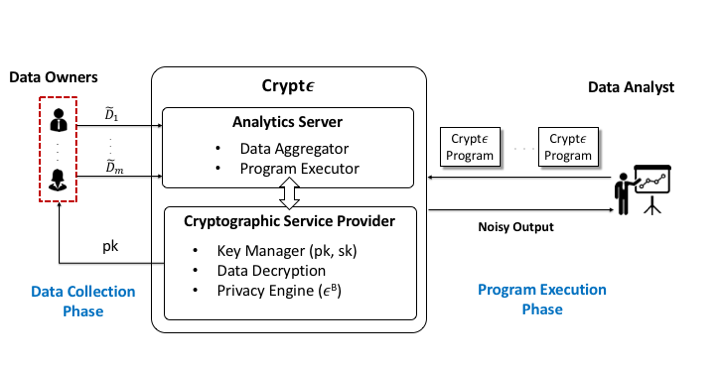
\includegraphics[width=\columnwidth]{diag.png}\caption{ Crypt$\epsilon$ System Setting: The  \textsf{AS} runs the Crypt$\epsilon$ programs. The \textsf{CSP} manages the cryptographic primitves. } \end{figure}
This section provides an overview of \system. We begin this section with the desiderata for \system that motivates our design followed by a discourse on the different components of \system and their functionality. Next we discuss about a few additional architectural choices we make for \system. This is followed by a description of \system's trust model and security sketch.

\subsection{Crypt$\epsilon$ Design}
The  desiderata for  the functionality of \system are as follows
\squishlist \item The architecture of \system should be able to support any differentially private algorithm that is permitted in the \textsf{CDP} model at the same order of accuracy guarantee as that of \textsf{CDP}, i.e. constant $O(\frac{1}{\epsilon})$ error bound.
\item Raw data records cannot be stored in the clear in any server, i.e., the server(s) in \system are untrusted. 
\item Data owners must be  off-line.\squishend
Recall from our discussion in section 1, \textsf{CDP} gives constant error bounds, however it relies on a trusted server for this. In contrast \textsf{LDP} requires no trusted server but results in limited accuracy.  The first two principles thus capture \system's objective of achieving the "best of both worlds", i.e., the accuracy guarantees and expressibility of the \textsf{CDP} model with  trust assumptions similar to that of the \textsf{LDP} model. The third principle stems from the fact that another undesirable trait of \textsf{LDP} is its inherent requirement for the data owners to be on-line during every query processing.  It is so because  in \textsf{LDP} %the private data of the individuals are not collated at a single place and hence%
depending on the query at hand, every time the data owners need to compute a different noisy measurement that best answers it. This is in general a poor practice as maintaining active communication channels for all the data owners might be unwieldy. \par The first desideratum can be achieved if we collate the data into a single data set such that any measurement can be performed on the entire data set at once followed by a single  instance of noise addition as opposed to aggregation over noisy measurements on individual data. The second desideratum mandates that the data hence collected should be suitably protected via cryptographic primitives (e.g. encryption scheme). Thus the first two requirements combined, necessitates \system to be able to perform differentially private computations on the encrypted data itself. This leads us to use linear homomorphic encryption and secure computation (specifically Yao's garbled circuits)  as the cryptographic primitives of our choice for \system. Note, by virtue of secure computation, we can potentially implement all the functionalities of the \textsf{CDP} model in \system. However, bearing the practical efficiency of the cryptographic primitives in mind, we impose certain limitations on the expressibility of \system. Due to the third desideratum, a generic $m+1$ party secure computation is ill-suited for our setting. This requires a third party entity that can factor out the onus of participating in a secure computation protocol from the data owners and capture its functionality in (at least) a 2-party protocol instead.   Moreover, since the data owners are no longer in the loop to monitor every query answering, the aforementioned entity should also watchdog the overall privacy budget expenditure. 
Guided by the above principles we design a two-server model for \system with the following components
\\(1)\textbf{ Data-Owners (\textsf{DO})} -  Each data-owner $\textsf{DO}_i, i \in [m]$ has  a
private data record $D_i$ and is willing to share it only if encrypted.   \\(2)\textbf{ Analytics Server (\textsf{AS})} - The \textsf{AS} wants to run a set of differentially private programs on the dataset $\mathcal{D}=\bigcup_{i=1}^m D_i$  but has 
access only to the encrypted copies of $D_i, i \in [m]$.
\\(3)\textbf{ Cryptographic Service Provider (\textsf{CSP})} -
 The \textsf{CSP} manages the cryptographic primitives used in Crypt$\epsilon$ and interacts with the \textsf{AS} to compute the
noisy answers. It is also responsible for monitoring the overall privacy budget expenditure.
%\xh{Rather than providing all the encryption details, can we just simply have an algorithm box to summarize the interactions between these three components. Then describe the interactions and highlight the key functionalities of each component, and then the trust model. }

 
 
\subsection{Crypt$\epsilon$ Modules}

\stitle{Cryptographic Service Provider (\textsf{CSP})}\\
(1)\textbf{ Key Manager }- The foremost duty of the \textsf{CSP} is to initialize the encryption scheme of Crypt$\epsilon$. This task is handled by the \textit{Key Manager} module which generates the key pair $(sk,pk)$ for the \textsf{labHE} scheme. It stores the secret key, $sk$ with itself and releases the public key, $pk$. Note that since the \textsf{CSP} has exclusive access to the secret key $sk$, it is the only entity capable of decryption in Crypt$\epsilon$.\\
(2)\textbf{ Data Decryption }- The \textsf{CSP} being the only entity capable of decryption,  any measurement of the data (even noisy) has to involve the \textsf{CSP}. The \textit{Data Decryption} module is tasked with handling all such interactions with the \textsf{AS}. \\
(3)\textbf{ Privacy Engine }- Crypt$\epsilon$ starts of with a total privacy budget of $\epsilon^B$ which is unanimously agreed upon by all the data owners. Note that the mechanism of deciding $\epsilon^B$ should be piloted by social prerogatives \cite{e1,e2} 
and is currently outside the scope of Crypt$\epsilon$. For executing any program, the \textsf{AS} has to interact with the \textsf{CSP} at least once (for decrypting the noisy answer) thereby giving the \textsf{CSP} the opportunity to monitor the \textsf{AS}'s actions in terms of privacy budget expenditure. The \textit{Privacy Engine} module hence maintains a public ledger that records the privacy budget spent in executing each program. Once the privacy cost incurred reaches 
$\epsilon^B$, the \textsf{CSP} refuses to decrypt any further answers thereby ensuring that the privacy budget is not exceeded.  The ledger is completely public allowing any data owner to verify it as and when desired.\\
\stitle{Data Owners (\textsf{DO})}\\
(1)\textbf{ Data Encoder} -  Each data owner $\textsf{DO}_i, i \in [m]$ has a private data record $D_i$ of the form $\langle A_1,...A_l\rangle$ where ${A}_j$ is an attribute. At the very outset, every data owner  $\textsf{DO}_i$ represents his/her private record $D_i$ in its respective per attribute one-hot-coding format. The one-hot-coding is a way of representation for categorical attributes and is illustrated by the following example. 
If the database schema in \system is given by  $\langle Age,Gender\rangle$ then corresponding one-hot-coding representation for a data owner $DO_i, i \in [m]$ with the record $\langle 30, Male\rangle$, is given by $\tilde{D_i}=\langle[\underbrace{0,\ldots,0}_{29},1,\underbrace{0,\ldots,0}_{70}],[1,0]\rangle$. \\
(2)\textbf{ Data Encryption} - The \textit{Data Encryption} module stores the public key $pk$ of the labHE scheme used in Crypt$\epsilon$ which is announced by the CSP. This key is used for an element-wise encryption of the data owner's  record of per attribute one-hot-codings. In our aforementioned example, we get $\mathbf{\tilde{D}}=\langle[\underbrace{labEnc_{pk}(0),\ldots}_{29},labEnc_{pk}(1),\\\underbrace{\ldots,labEnc_{pk}(0)}_{70}],
[labEnc_{pk}(1),labEnc_{pk}(0)]\rangle$. Finally the data owner sends this encrypted record to the \textsf{AS} via a secure channel. This is the only interaction that a data owner ever participates in, all the program executions are carried out by the \textsf{AS} and the \textsf{CSP} with the data owners being completely off line.\\
\stitle{Analytics Server (\textsf{AS)}}\\
(1)\textbf{  Aggregator} - The \textit{Aggregator} collects the encrypted records $\mathbf{\tilde{D_i}}$ from each of the data owners $\textsf{DO}_i$ and collates them into a single encrypted database $\boldsymbol{\tilde{\mathcal{D}}}$. %Note that in contrast, the server in the \textsf{CDP} model, being trusted, stores the data in the clear whereas in the \textsf{LDP} model the untrusted server stores appropriately randomized (noisy) data.   
\\(2)\textbf{ Program Executor }- The \textit{Program Executor} is the most important module of the \textsf{AS} and is tasked with the execution of Crypt$\epsilon$ programs. It takes as input a Crypt$\epsilon$ program from an external data analyst, alongside the appropriate privacy parameter $\epsilon$ and publishes the differentially private output computed with the assistance of the \textsf{CSP}. Crypt$\epsilon$ supports a set of 9 primitives and a Crypt$\epsilon$ program is an execution plan expressed as a sequence of these primitives. The primitives can be broadly classified into two types- transformation primitives and measurement primitives. Transformation primitives allow certain modifications on the encrypted data and are performed almost entirely by the \textsf{AS}. The measurement primitives on the other hand reveal some noisy measurement of the data and requires interaction with the \textsf{CSP}. \system supports two types of measurement primitives that implement two of the most popular differentially private mechanisms, Laplace mechanism \cite{Dork} and Noisy-Max \cite{Dork}. A typical Crypt$\epsilon$ program execution consists of  a series of transformation on the encrypted data followed by a measurement primitive and arbitrary post-processing. \\
 \textit{Noise Addition in \system} - For the Laplace mechanism, both the \textsf{AS} and the \textsf{CSP} add two separate instances of the random noise to the program output. This is necessary because had only one of them added the noise, then after the release of the clear text output, that party can simply subtract out the noise to reveal the true private answer. An alternative way can be both \AS and \CSP jointly computing a single instance of the noise using a secure computation protocol (see Appendix D.1). However, we do not implement it in the current version of \system as the two-fold noise addition is more efficient. For the Noisy-Max primitive, we provide an efficient secure computation protocol where only a single instance of noise by either party suffices. 
Since in Crypt$\epsilon$ the point of noise addition is just at the two servers, unlike at every individual in \textsf{LDP}, we achieve constant error bounds which is of the same order as that of \textsf{CDP} (see section \ref{exp:results}). 
\subsection{Crypt$\epsilon$ Workflow}
The complete workflow of Crypt$\epsilon$ is outlined as follows\\(1) \textbf{ Setup Phase} - This is the very first step in Crypt$\epsilon$ where the key manager of \textsf{CSP} generates the key pair for labHE $(sk,pk)$, publishes $pk$ and stores $sk$. \\(2) \textbf{ Data Collection Phase }- In the next phase, the $\textit{Data 
Encoder}$ and $\textit{Data Encryption}$ modules of every data owner, work to produce the encrypted data records which are then submitted to the \textsf{AS}. The data owners are relieved of all other duties and can go completely off-line. The $\textit{Aggregator}$ module of the \textsf{AS} then aggregates these encrypted records into a single encrypted database $\boldsymbol{\tilde{\mathcal{D}}}$. \\(3) \textbf{ Program Execution Phase} - In this phase, the \textsf{AS} executes a Crypt$\epsilon$ program with some interaction with the \textsf{CSP}  and generates a differentially private output.  \\
The \emph{Setup} and \emph{Data Collection} phases occur just once at the very beginning, every subsequent program  is handled via the corresponding  \emph{Program Execution} phase. Figure 1 shows the diagrammatic representation of \system. A comparative analysis of \system, \textsf{CDP} and \textsf{LDP} is presented in  Table \ref{DPCompare}.
\begin{table}[h!]
\centering
\caption {Comparative analysis of the different DP models \am{LDP does not have a data curator. Maybe a better way to put it is: Centralized Server: Yes/No. Trust assumption on Central Server: NA for LDP; Trusted for CDP and Untrusted/Non colluding for Crypte. Again Data storage in central server should be NA for LDP. Adversary should be Info.Theoretic for LDP and CDP and Computationally bounded for Crypte? Error should be Error on statistical counting query? I do not know about the impossibility result section. We need a tighter charaterization for CDP and Crypte. For instance, one can not learn a threshold function under CDP, but I would not call it unbounded sensitivity. I would drop the last line.  }}
\scalebox{0.6}{ \begin{tabular}{|l| c c c|}  \toprule
\multicolumn{1}{|c}{\textbf{Features}} & \textbf{LDP}  & \textbf{CDP}  & \textbf{Crypt$\epsilon$}  \\ [0.5ex] 
 \hline \hline\# Servers & 1& 1 & 2\\\hline
Trust  & & & Untrusted \\  Assumption & Untrusted & Trusted & Semi Honest \\for Server &  &   &  Non-Colluding  \\ \hline
Data Storage & \multirow{2}{*}{Noisy} & \multirow{2}{*}{Clear} & \multirow{2}{*}{Encrypted} \\in Server & &  &  \\\hline
Adversary & Unbounded & Unbounded & Bounded \\\hline
 Error & $O\Big(\frac{\sqrt(n)}{\epsilon}\Big)$& $O\Big(\frac{1}{\epsilon}\Big)$ & $O\Big(\frac{1}{\epsilon}\Big)$\\\hline
 Impossibility & Everything & Algorithms w/ & Same as that \\results & beyond SQ model & Unbounded Sensitivity & of \textsf{CDP} in theory \footnotemark\\
  [1ex] 
 \bottomrule
 \end{tabular}}\label{DPCompare}
\end{table}
\footnotetext{For practical constraints the current implementation has restrictions}
 %in between that of the central differential privacy model and the local differential privacy model - although it is definitely much weaker than that of the central differential privacy model, Crypt$\epsilon$'s trust model is slightly stronger as compared to that of the local differential privacy model owing to the aforementioned premises. 
%The formal security analysis for \system is presented in Appendix section B. 
\begin{comment}
learn any other information about the private datasets Di beyond what is revealed by the
model itself. Even in the case that one of the two servers (MLE or CSP) colludes with some
of the data-owners, they should learn no extra information about the data held by the
honest data-owners. In order to achieve this goal we design a system that can be seen as
multi-party protocol run by the m +2 parties mentioned before and specified by a sequence
of steps. This system (described in Section 4) has the following two-phase architecture:
We assume that the Evaluator and the CSP do not
collude. Each one may try to subvert the system as
discussed above, but they do so independently. More
precisely, at most one of these two parties is malicious:
this is an inherent requirement without which security
cannot be achieved.
• We assume that the setup works correctly, that is all
users obtain the correct public key from the CSP. This
can be enforced in practice with appropriate use of
Certificate Authorities.
Note that is true for any cryptographic primitive and is 
The can actually be avoided by removing the . m+1 secure computation where However this is Thus by capturing the we are having an huge efficincy gain now that teh problem is reduced to antwo-party

\subsection{Protocols} \xh{This might go first with the algorithm box or figure.}
In this section, for each of the three entities we list down the interactions that are initiated by them.
\begin{itemize}\item CSP- The foremost duty of the CSP is to initialize the encryption scheme of Crypt$\epsilon$. Specifically the CSP generates the key pair $(sk,pk)$ for the labeled homomorphic encryption. It stores $sk$ with itself and makes $pk$ public. Note that since only the CSP has access to the secret key $sk$, it is the only entity capable of decryption in Crypt$\epsilon$.
\item Data owners- Recall that each data owner owns a single private record which he/she shares with the AS in the encrypted form as follows. First every data owner represents his/her record in its respective per attribute one-hot-encoding format. For example, if the database schema is given by  $D=<Age,Gender>$ then a data owner with the record $<30, Male>$ would firstly represent it as $\mathcal{E}(D)=<[\underbrace{0,\ldots,0}_{29},1,\underbrace{0,\ldots,0}_{70}],[1,0]>$. This is followed by an element-wise encryption of this record of per attribute one-hot-encodings using the pubic key $pk$. In our aforementioned example, we get $\mathbf{D}=<[\underbrace{Enc(0),\ldots}_{29},Enc(1),\underbrace{\ldots,Enc(0)}_{70}],[Enc(1),Enc(0)]>$. Finally the data owner sends this encrypted record to the AS. Note that this is the only interaction that a data owner ever participates in. All the  query answering are carried out by the AS and the CSP with the data owners being completely off line. \item AS - After receiving the encrypted records from each of the data owners, the AS first collates them into a single encrypted database $\mathbf{\tilde{D}}$. For any subsequent query answering, $\mathbf{\tilde{D}}$ is subjected it to a series of transformations most of which are carried out by the AS by itself. However since the CSP is the only entity capable of decryption, for getting any measurement (even noisy) in the clear the AS has to interact with it. There are precisely two types of interactions between the AS and the CSP \begin{enumerate}\item Yao's Garbled Circuit \item Decryption of encrypted noisy value\end{enumerate}\end{itemize}
\end{comment}


\eat{Yet another alternative implementation could have been to engage the $m$ data owners and the \textsf{AS} in a $m+1$ secure computation protocol. This approach has two disadvantages. Firstly, as the number of data owners grow, the communication and computation overheads of this $m+1$ secure computation protocol would get prohibitively high. Secondly, this violates our requirement of off-line data owners. Thus by introducing a separate entity in the form of the \textsf{CSP}, we factor out the onus of participating in a secure multi party computation from the data owners and capture their computation power in a secure protocol between just the \textsf{CSP} and the \textsf{AS} instead %. Note that with the \textsf{CSP} in the picture, the secure computation is now reduced to a two-party case
irrespective of the number of data owners. %Not only does this improve the efficiency of our protocols drastically but is also advantageous from the perspective of ease of system implementation and maintenance. It is so because otherwise we would have had to maintain secure channels between all pairs of data owners, which would become extremely cumbersome with large values of $m$. Moreover all the data owners would have to be online for every program execution. Hence the choice of having a separate server in the form of the \textsf{CSP} is made from the efficiency point of view.
%The second assumption of an computationally bounded adversary is inherent in semantically secure cryptographic protocols. %Another design choice for Crypt$\epsilon$ could have been to keep the data owners in the loop for every program execution such that some of the data transformations could be pushed down to them. Since the data owners can perform the transformations on the plain text and in parallel, this could potentially improve performance. However this would require the data owners to be on-line during the program execution which might be unwieldy in practice especially with a large number of geographically dispersed data owners. 
\par %Keeping the efficiency of our implementation in mind, we used only two instances of simple two-party Yao's garbled circuits for Crypt$\epsilon$. In addition, we propose two optimizations that leverage on the fact that the \textsf{AS} is satisfied with differentially private outputs; this allows  us to expend some of the privacy budget in differentially private pre-processing of the encrypted data. 
The class of programs supported by Crypt$\epsilon$ is any program that can be expressed as a composition of  Crypt$\epsilon$ primitives followed by arbitrary post-processing. Crypt$\epsilon$ supports 7 transformation primitives and 2 measurement primitives. The noisy measurements allowed are the Laplace mechanism and the Noisy max (see section 4.2), two of the most popular and standard differentially private algorithms. The main constraint behind the design of the transformation primitives is that their composition should allow seamless sensitivity analysis.  Sensitivity analysis of arbitrary relational algebraic queries is a hard problem, for e.g. sensitivity of conjunctive counting queries with join operator is unbounded \cite{sensitivity}. Hence all the transformations that Crypt$\epsilon$ supports have bounded stability \cite{PINQ} such that the sensitivity analysis of any program written using them is straightforward. In fact, we showcase that the proposed Crypt$\epsilon$ primitives are indeed very powerful, enabling us to answer practically useful queries, such as linear counting queries etc. 
\\ 
}





\subsection{Trust Model}
Both the servers, \textsf{AS} and \textsf{CSP} are completely untrusted in Crypt$\epsilon$. 
Thus from the data owners perspective the trust assumption is similar to that of \textsf{LDP}; the data owners need not place their trust in any external entity. 
However there are two modest differences in the Crypt$\epsilon$ setting from that of \textsf{LDP}.\\
 (1) We assume that the \textsf{AS} and the \textsf{CSP} are non-colluding and follow the \emph{honest-but-curious} (or \textit{semi-honest}) adversary model. %That is, they always follow the instructions of the protocol faithfully but strive to learn extra information about the private records from the messages received during the execution of the protocol. 
 Moreover we assume that each data owner has a private channel with the \textsf{AS}. This is to prevent any third party (including the \textsf{CSP}) from eavesdropping. \\
 (2) The adversary is now reduced to a \textit{computationally bounded} one as opposed to the information theoretic one  in \textsf{LDP}.
 

 \subsection{\system Security Sketch}
 Let $\Pi$ represent the protocol for the end-to-end execution of a $\epsilon$-DP program in \system.  In this paper we consider a
semi-honest adversary  $Adv$ (see section 3.4) who can corrupt any subset of the data owners, the data analyst and at most one of the two
servers. This captures our assumption that the two servers are non-colluding. Thus the requisite security definition should state that $Adv$ only learns the data of the corrupted data owners and the differentially private output but nothing else about the honest data owners. In other words, the view of the adversary $Adv$ should be \emph{computationally indistinguishable} from a truly differentially private protocol. 
Let $P$ be a program that is submitted by the data analyst to the protocol $\Pi$ and it is to be run on the data set $\mathcal{D}$ with the privacy parameter $\epsilon$. Thus based on our discussion on noise addition in sec 3.2, we define the ideal functionality $\mathcal{F}=(\mathcal{F}_1,\mathcal{F}_2)$ of the protocol $\Pi$ as follows.
\\If $P$ uses Laplace mechanism \cite{Dork}, then
\begin{gather} 
\mathcal{F}_1(P,\mathcal{D},\epsilon)=P(\mathcal{D})+\eta_2\\\mathcal{F}_2(P,\mathcal{D},\epsilon)=P(\mathcal{D})+\eta_1 \\ \eta_1, \eta_2 \sim Lap(\frac{\Delta}{\epsilon})\end{gather}  where  $\Delta$  is the suitable sensitivity of the program. In this case, $output^{\Pi}(P,\mathcal{D})$ which denotes the published output of \system, is given by $P(\mathcal{D})+\eta_1+\eta_2$.\\
If $P$ uses Noisy-Max mechanism \cite{Dork}, then
\begin{multline}
\mathcal{F}_1(P,\mathcal{D},\epsilon)=\mathcal{F}_2(P,\mathcal{D},\epsilon)=Noisy-Max(P(\mathcal{D}),\Delta,\epsilon) 
\end{multline} where $P(\mathcal{D})$ produces a vector and  $\Delta$ is the suitable sensitivity of the program. $output^{\Pi}(P,\mathcal{D},)$ in this case is equal to $Noisy-Max(P(\mathcal{D}),\Delta,\epsilon)$.\\
Formally, using the standard simulation based definition \cite{Oded},
\begin{theorem}  Let $S \subset \{1,...,m\}$ then $\Pi$, (i.e. the protocol for an end-to-end program execution in \system) realizes $\mathcal{F}$ (eq 3-6)  with correctness and privacy against
the adversaries $Adv_1=\textsf{AS} \cup \{\textsf{DO}_i, i \in S\} \cup \mbox{Data Analyst}$  and $Adv_2=\textsf{CSP} \cup  \{ \textsf{DO}_i, i \in S\} \cup \mbox{Data Analyst}$
 if there exists  P.P.T algorithms $Sim_1$ and $Sim_2$ such that  \begin{align*}
 \big\{Sim_1({D_i, i \in S},\mathcal{F}_1(P,\mathcal{D},\epsilon)),\mathcal{F}(P,\mathcal{D},\epsilon)\big\} &\\\stackrel{C}{\equiv} \big\{view^{\Pi}_{Adv1}(P,\mathcal{D}),output^{\Pi}(P,\mathcal{D})\big\}  \numberthis\label{adv1}
               \\
 \big\{Sim_2({D_i, i \in S},\mathcal{F}_2(P,\mathcal{D},\epsilon)),\mathcal{F}(P,\mathcal{D},\epsilon))\big\} &\\\stackrel{C}{\equiv}\big\{ view^{\Pi}_{Adv2}(P,\mathcal{D}),output^{\Pi}(P,\mathcal{D})\big\}  \numberthis\label{adv2}
\end{align*} for all possible inputs  where $ \stackrel{C}{\equiv}$ denotes computational indistinguishability and $view^{\Pi}_i$ denotes the view of entity $i$ in protocol $\Pi$. 
\end{theorem}
\begin{corollary} Protocol $\Pi$ satisfies \textsf{SIM-CDP} \cite{CDP} privacy.\end{corollary}
The proof of this is presented in Appendix A. \eat{Here we just present an intuitive understanding of it. The interactions between the \textsf{AS} and the \textsf{CSP} can be categorised as \\(1) \textsf{CSP} generates garbled circuits with noisy outputs that are evaluated by the \textsf{AS}\\(2) \textsf{AS} sends encrypted masked data to the \textsf{CSP} and gets a transformed encrypted data in response \\(3)\textsf{AS} sends encrypted noisy data and gets back the data in the cleat with additional noise from the \textsf{CSP}\\
The garbled circuits are inherently semantically secure. For the second type of interaction, the random
mask hides the true plaintext
from the \textsf{CSP} while the \textsf{AS} cannot decrypt anything as it does not have access to the secret key $sk$. The last type of interaction outputs a noisy measurement over the data and illustrates the fact that both  \textsf{AS} and \textsf{CSP} add noise to the final answer in \system to ensure that both the servers are allowed only a differentially private  view of the data. Moreover, in
addition to the \emph{Program Executor} module of the \textsf{AS}, the data analyst
communicates the \system program and the privacy parameter $\epsilon$
to the \textit{Privacy Engine} module of the \textsf{CSP}. This enables the \textsf{CSP} to
compute the sensitivity of the program for itself (required while
adding its own noise) thereby thwarting any privacy budget over
expenditure attempts.}
 




\subsection{Discussion on Crypt$\epsilon$ architecture}\label{architecture}
 Crypt$\epsilon$  is based on the premise that there are $m$  data owners, each possessing a private data record, and the \textsf{AS} is the primary entity who is interested in learning certain differentially private statistics on the collective data.  Thus in \system, we require the \textsf{AS} to  shoulder the major chunk of the workload for any Crypt$\epsilon$ program execution; interactions with the \textsf{CSP} should be minimal and only related to data decryption.
Keeping this in  mind, we design the \textsf{AS} to perform most of the data transformations by itself (Table \ref{perf}). Specifically for every Crypt$\epsilon$ program, the \textsf{AS} processes the whole database and transforms it into concise representations (like an encrypted scalar or a short vector) which is then decrypted with the help of the \textsf{CSP}. It is interesting to note that we could have had an alternative implementation for Crypt$\epsilon$ where the private database is equally shared between the two servers and they engage in a secret share based secure computation protocol for computing the differentially private answers. However, this would require both the servers to do almost equal amount of work for every program. Such an arrangement would be justified only if both the servers are equally invested in learning the differentially private statistics and is ill-suited for Crypt$\epsilon$. Additionally, a secret-share based computation would be much more communication intensive resulting in a performance hit. 

The primitives for \system have been designed bearing two things in mind. Firstly, their composition should allow easy sensitivity analysis (for e.g. transformations must have bounded stability). Secondly, all the primitives should have very efficient implementations. Thus although the architecture of \system imposes no fundamental restriction on its expressibility and in theory we can enjoy the same algorithmic power as that of \textsf{CDP}, we restrict the expressibility in the current implementation of \system to ensure practicality of \system programs. Nevertheless, there is a separation between \system and \textsf{LDP} as explained in Appendix D2.


\eat{\begin{table}[h!]
\small
\centering
\caption {Comparative analysis of the different DP models}
 \begin{tabular}{l| c c c}  \toprule
\multicolumn{1}{c}{\textbf{Features}} & \textbf{LDP}  & \textbf{CDP}  & \textbf{Crypt$\epsilon$}  \\ [0.5ex] 
 \midrule \midrule \# Servers & 1& 1 & 2\\\hline
Trust  & & & Untrusted \\  Assumption & Untrusted & Trusted & Semi Honest \\for Server &  &   &  Non-Colluding  \\ \hline
Data Storage & \multirow{2}{*}{Noisy} & \multirow{2}{*}{Clear} & \multirow{2}{*}{Encrypted} \\in Server & &  &  \\\hline
Adversary & Unbounded & Unbounded & Bounded \\\hline
 Error & $O\Big(\frac{\sqrt(n)}{\epsilon}\Big)$& $O\Big(\frac{1}{\epsilon}\Big)$ & $O\Big(\frac{1}{\epsilon}\Big)$\\\hline
 Impossibility & Everything && \\results & beyond SQ model & None & None\footnotemark\\
  [1ex] 
 \bottomrule
 \end{tabular}
\end{table}
\footnotetext{Theoretically no restriction, however practical constraints maybe present}}

%\arc{ Can add another column for Mixnets maybe?}

\input{security_sketch}

\section{Use Cases}
\subsection{DPBench algorithms}
\paragraph{\textbf{AHP}}- Zhang et al in \cite{AHP} outline a state-of-the-art technique for  publishing differentially private histogram.  They introduce a new clustering (or grouping) framework which evaluates 
the trade-off between the approximation error due to clustering
and the Laplace error due to Laplace noise injected. This results in significant improvements in the accuracy of the sanitized histograms as compared to existing results.

\paragraph{\textbf{MWEM}}- In this  paper \cite{MWEM}, Hardt et al  combine the Exponential Mechanism with the Multiplicative Weights update rule \cite{MW} to produce a synthetic database that
substantially improves the performance of differentially private linear queries. The Multiplicative Weights is an iterative approach  maintaining and correcting an approximate distribution through queries  on which the approximate and true datasets
differ. The Exponential Mechanism, in this context, selects the queries that are most incorrect with respect to the current approximation. 
\am{MWEM, AHP, DAWA, type algorithms can be implemented}
\subsection{Learning}\label{Learning}
\paragraph{\textbf{Linear Regression}}-
A linear regression is a supervised learning algorithm  that assumes a linear relationship between a quantitative outcome and a set of quantitative explanatory variables. Specifically, on an input of
n points $\{(x_1, y_1), ... , (x_n , y_n)\}$ (where $x_i \in \mathcal{R}^d 
$ and $y_i \in \mathcal{R} $), the algorithm outputs a vector $w* \in \mathcal{R}^d
$
such that $w*|
x_i \approx y_i \forall i \in \{1,...,n\}$. The computation of $w$ is done by minimizing a linear combination of a loss function and a regularization term, that
is, $w* \in \arg\min_{w \in R^d} f_{X,y}(w) + \lambda R(w) $ where $\lambda \geq 0$ is fixed. A popular and convenient loss function is the squared loss function  which penalizes the
residual of the prediction quadratically, $f_{X,y}(w)=||Xw-y||_2^2$. Here $X \in \mathcal{R}^{n\times d}$
is the matrix with the vector $x^T_i$ as $i^{th}$ row and $y \in R^n$
is the vector with the value $y_i$ as $i^{th}$ component. We assume
that X is always full rank (i.e., $rk(X)=d$). The regularization term is
added to avoid over-fitting the training dataset and  prevents the weights from getting too large. In
practice, one of the most common regularization terms is the 2-norm $(R(w)=||w||_2^2)$ which
generates a model with overall smaller components. Such a model is called the ridge regression and is computed by minimizing the function $F_{ridge}(w)=||Xw - y||_2^2+ \lambda ||w||_2^2$. Since,
$\Delta F_{ridge}(w) =2X^T(Xw - y) + 2\lambda w$,  $w*$
can be computed by solving the linear system
\begin{gather}Aw =b \end{gather}
where $A=X^TX + \lambda I$ (symmetric $d \times d$ matrix) and $b= X^Ty$ (vector of d components).
Notice that since X is full-rank, A is positive definite and therefore $det(A) > 0$ (in particular
A is invertible).
\\ In this section, we illustrate how to adapt the computation of a differentially private linear regression model to our proposed protocols. The AS is the machine learning engine (MLE) in our context. The CSP and the $m$ data owners $ DO_1,... , DO_m$ remain unchanged
 as in \cite{LReg}. For the collection of data from the data owners and the subsequent privacy preserving computation, we are using the model as proposed in \cite{LReg}. For the appropriate noise to be added to achieve differential privacy, consider the following discussion.\\
\textbf{Definition  (L2-sensitivity)}. Assume that  $f$ is a deterministic query that maps a dataset to a vector in $R^d$. The L2-
sensitivity of $f$ is defined to be $\Delta_2(f ) = \max_{S\sim S'}
||f (S) - f (S')||$ where $S$ and $S'$ are neighboring datasets.
The following theorem relates $\epsilon$-differential privacy and L2-sensitivity.

\textbf{Theorem}\cite{sensitivity} Let $f$ be a deterministic query that maps a database to a vector in $R
^d$
. Then publishing $f (D)+\eta$
where $\eta$ is sampled from the distribution with density
\begin{gather}p(\eta) \propto  exp\Big(-\frac{\epsilon||\eta||}{\Delta_2(f)}\Big)
\label{noise}
\end{gather}
ensures $\epsilon$-differential privacy.\\\\\\
Notations:
\arc{Ideally these would be explained in details earlier in the paper depending on the LHE scheme we use. I am temporarily including it here for ease of readability.}
\\
$\mathcal{M}$ denotes the message space.\\
Let C be the set of all possible ciphertexts. Then $\odot$ represents an operation on C such that
for any a-tuple of ciphertexts $c_1 \leftarrow Enc_{pk}(m_1), ... , c_a \leftarrow Enc_{pk}(m_a)$ (a positive integer), it
holds that $Pr\Big[Dec_{sk}(c_ \odot ... \odot c_a) = m_1 +... + m_a\Big]  =1$. Also $cMult(a,c)=c\odot...\odot c$(a times). \\  Here we use of \textit{labeled-homomorphic encryption}, labHE which can be constructed from a LHE and a pseduorandom function. The operation $labMult(c, c')$ works as follows. On input two labeled ciphertexts, $c  (a, c)$ and $c'=(a',c')$ 
 it computes a
“multiplication” ciphertext $d  =labMult(c, c')$ as  as $ d =Enc_{pk}(a \cdot a')\odot cMult(a, c')\odot cMult(a',c)$.\\\\\\\\
The protocol works as follows
\\ \textbf{Parties:} \textit{ CSP, AS, and }$DO_k$ \textit{ with input } $D_k, \forall k \in \{1,...m\}$\\
\textbf{Output:}  \textit{ AS gets A' and b'
(i.e., encryptions of A and b, respectively).}\\
\textbf{Step 1: } \textit{ (key-generation) CSP runs  }$(sk, pk) \leftarrow Gen(\kappa) $\textit{ and makes } $pk$ \textit{ public,}\\ \textit{    while it keeps } sk \textit{ secret.}\\
\textbf{Step 2:} \textit{ (local computation) } $\forall k \in \{1,...,m\}   DO_k$
\textit{computes } $A_k=\sum_ix_i^Tx_i$ \text{ and } $b_k=\sum_iy_ix_i$ \textit{ with } $n_{k-1}+1 \leq i\leq n_k$; next $DO_k$ encrypts $A'$
\textit{ next, }$DO_k$ \textit{ encrypts them, } $A'_k[i,j]=Enc_{pk}(A_k[i,j]), b'_k[i]=Enc_{pk}(b_k[i]), \forall i,j \in \{1,...,d\}, j\geq i$; \textit{ finally } $DO_k$ \textit{ sends all } $A'_k$ \textit{ and } $b'_k$ \textit{ to AS }.
\\
\textbf{Step 3:} \textit{(datasets merge) }\begin{gather*}A'[i,j]=\begin{cases}\Big(\bigodot^m_{k=1}A'_k[i,i]\Big)\odot Enc_{pk}(\lambda) &\mbox{ if } j=i\\\bigodot_{k=1}^m A'_k[i,j] &\mbox{ if } j > i\end{cases},b'[i]=\bigodot_{k=1}^m b'_k[i]\end{gather*}
\\\textbf{Step 4:} \textit{ AS computes the differentially private regression model using } \\\textbf{Protocol - 1}.
\\ \textbf{Step 4a:}\textit{(data masking) AS samples a random invertible matrix } $R \in GL(d,Z_N)$ \textit{ and a random vector } $r \in Z_N$ \textit{ and } $\eta$ \textit{ from the distribution  } \eqref{noise} \textit{ and it uses the linear homomorphic property of the underlying encryption
scheme to compute } $C'= Enc_{pk}(AR)$ \textit{ and } $g'=Enc_{pk}(b + A(r+\eta))$. \textit{ The values } $C'= AR$ \textit{ and } and
$g'=  b + A(r+\eta)$ are the “masked data.” Specifically the performs the following operation \begin{gather*} C'[i,j]=\bigodot^d_{k=1}cMult(R[k,j],A'[i,k])\\g'[i,j]=b'[i]\odot\Big(\bigodot^d_{k=1}cMult(r[k]+\eta[k],A'[i,k])\Big)\end{gather*}
$\forall i,j \in\{1,...,d\}$; next AS sends $C'$ and $d'$ to CSP.
\\\textbf{Step 4b: }\textit{(masked model computation)}
\textit{ The CSP decrypts } $C'$ \textit{ and }$g'$ \textit{ and computes }$\tilde{w}=  C^{-1}g$. \textit{ The vector w is the “masked
model” sent back to the AS.}
 \\\textbf{Step 4c:} \textit{(model reconstruction) The AS computes the desired model as } $w =R\tilde{w} - r$. \textit{ Indeed, it is easy to verify that}
\begin{gather*}R\tilde{w} - r =R\big(AR)^{-1}(b+A(r+\eta)\big)-r\\=A^{-1}b+\eta
\end{gather*}
\subsection{Example Queries}
In this section we illustrate four working examples for our proposed protocols.\\ Let us assume that every data owner $DO_k, k \in\{1,...,m\}$ holds a two-tuple in \textit{Age}$\times$\textit{Gender}. Recall that the chosen representation for our values is one-hot-coding. Let $Gender^k_{Enc}$ and $Age^k_{Enc}$ denote the ciphers for the categories  gender and age respectively for the data owner $DO_k$.  Assume that for the category gender, male is encoded as bit string $10$ and female as $01$ and the age is an integer in $[1,...100]$. Thus the cipher for a female data owner of age 24 would be $Gender_{Enc}=[Enc_{pk}(0),Enc_{pk}(1)], Age_{Enc}=[\underbrace{Enc_{pk}(0),...,Enc_{pk}(0)}_\text{23},Enc_{pk}(1),\underbrace{Enc_{pk}(0),...,Enc_{pk}(0)}_\text{76}]$.   For the rest of the discussion, we assume that each data owner $DO_k$ communicates  his/her respective cipher pair $\{Gender^k_{Enc},Age^k_{Enc}\}$ to the AS beforehand.\\\\
\textbf{Query 1:} Drop the gender column and partition the age data into 100 bins, where the $i^{th}$ bin corresponds to age $i \in \{1,...,100\}$.  Design a mechanism to provide differentially private answers to queries of the form "Report the number of data owners with age less than equal to $i$".
\paragraph{Mechanism:} 
\begin{enumerate}\item First the AS simply ignores the cipher $Gender^k_{Enc}, \forall k \in \{1,...,m\}$. \item Next the AS performs a vector like addition (i.e., add corresponding components of the tuple together) of all the ciphers $Age^k_{Enc}, \forall k \in \{1,...,m\}$. Let $\mathcal{A}'$ be the resulting tuple, thus we have \begin{gather}\mathcal{A}'[i]=Age^1_{Enc}[i]\odot....\odot Age_{Enc}^m[i], i \in [1,...,100] \label{A}\end{gather} It is easy to see that $Dec_{sk}(\mathcal{A}'[i]) = \# \textit{ people with age = i}$.
\item In order to compute the number the people with age at most i, the AS performs $C'=\mathcal{A}'[1]\odot ...\odot \mathcal{A}'[i]$. Clearly $Dec_{sk}(C')=C=\#\textit{people with age at most i}$. \item Finally it uses the proposed \textbf{Protocol-1} as follows.\begin{enumerate}\item AS samples a random integral value $r \in \mathcal{Z}$ and and sends masked value $\tilde{C}'=C'\odot r$  to the CSP. \item The CSP decrypts $Dec_{sk}(\tilde{C}')=\tilde{C}=C+r$.  \item CSP sends noisy value $\hat{C}=\tilde{C}+\eta, \eta \in Lap(\frac{1}{\epsilon})$ to AS.  \item Finally AS subtracts $r$ from $\hat{C}$ to report the $\epsilon$-differentially private query response $C+\eta$.  \end{enumerate} \end{enumerate}
\textbf{Query 2:}Drop the gender column of the data and partition the age into 100 bins like before. Design a $\epsilon$-differentially private mechanism to report the age with the maximum count, i.e., mode.
\paragraph{Mechanism:}\begin{enumerate}\item AS ignores the ciphers $Gender^k_{Enc}, \forall k \in \{1,...,m\}$ and computes $\mathcal{A}'$ as in \eqref{A}. \item Next AS draws an uniformly random sample $\textbf{R} \in_R [\mathcal{Z}]^{100}$ and computes $\tilde{\mathcal{A}}'[i]=\mathcal{A}'[i]\odot\textbf{R}[i], i \in \{1,...,100\}$ \item AS sends $\tilde{\mathcal{A}}'$ to CSP and engages in \textbf{Protocol-2}. \begin{enumerate}\item First CSP decrypts $\tilde{\mathcal{A}}'$. \item Next the CSP constructs a garbled circuit that performs the following actions \\\textbf{Input}- CSP:$\eta \in [Lap(\frac{1}{\epsilon})]^{100}$; AS: R \begin{enumerate}\item Removes the mask $R$ from $\tilde{\mathcal{A}}$ to recover the corresponding $\mathcal{A}$
\item Injects laplacian noise to get $\hat{\mathcal{A}}=\mathcal{A}+\eta$ \item Outputs $\arg_{i}\max\{\mathcal{A}[i]\}, i \in \{1,...,100\}$  \end{enumerate}  The CSP subsequently makes the garbled circuit  and the garbled inputs corresponding to $\eta$ available
to the AS. \item Then, it engages in an oblivious transfer
protocol with the AS, so that the AS obtains garbled
values of the masks: $GI(R)$. 
\item Finally, the AS evaluates
the circuit, whose final (ungarbled) output comprises the
requested noisy max.\end{enumerate}
\end{enumerate}
\textbf{Query 3:}Partition the data first by gender and then by age in ranges of 10. Release the $\epsilon$-differentially private  count for each bin. \paragraph{Mechanism}For this we use the labeled homomorphic encryption scheme (labHE).
\begin{enumerate}\item AS generates two sets of "multiplication" ciphers 
′k,j[i]=labMult(GenderEnc[j],AgeEnc[i])j={1,2},k∈{1,...,m},i∈{1,...,100}
 Thus if data owner DOk is male then Decsk(Tk,2)[i]=0∀i∈{1,...,100} and Decsk(Tk,1) gives us the one-hot-code for the data owner's age. \item Next AS computes 
′j[i]=′1,j[i]⊙...⊙′m,j[i],j∈{1,2},i∈{1,...,100}
Hence Decsk(′1) and Decsk(′2)  gives us the count of the number of males and females respectively of age i. \item Then, the AS reduces the counts into ranges of 10 as follows
A′j[i]=′j[(i−1)∗10+1]⊙...⊙′j[i∗10],i∈{1,...,10}
\item Next AS follows \textbf{Protocol -1} to report the noisy counts for each of the 10 bins in Aj
\begin{enumerate}\item AS draws an uniformly random sample $R \in [\mathcal{Z}]^{10}$ and mask $\textbf{A}_j$ as $\mathbf{\tilde{A}}'_j=\textbf{A}_j[i]\odot R[i] i \in \{1,...,10\}$; AS sends $\mathbf{\tilde{A}}'_j$ to CSP.  \item The CSP decrypts $Dec_{sk}(\mathbf{\tilde{A}}'_j)=\mathbf{\tilde{A}}_j=\mathcal{A}_j+R$.  \item CSP sends noisy value $\hat{A}_j=\mathbf{\tilde{A}}_j+\eta, \eta \in [Lap(\frac{1}{\epsilon})]^{10}$ to AS.  \item Finally AS subtracts $R$ from $\hat{A}_j$ to report the $\epsilon$-differentially private query response $\textbf{A}_j+\eta$. \end{enumerate}
\end{enumerate} However the aforementioned mechanism results in 200 \textit{ labMult()} operations for each data owner driving up the computation costs. An alternative mechanism is outlined below.  Let us assume that each data owner now generates two ciphers E[1:] and E[2:] which represent either a 0-vector or the age in one-hot-coding based on the gender of DOk. If the gender of data owner DOk is male and age \textbf{i} 
Ek[1,i]=Encpk(1)Ek[1,i]=Encpk(0)∀i∈{1,...,100},i≠iEk[2,i]=Encpk(0)∀i∈{1,...,100}
 The cipher for female data owners are generated similarly. 
\begin{enumerate}\item AS computes \begin{gather}\mathcal{A}'_j[i]=E^1[j,i]\odot ...\odot E^m[j,i], j \in \{1,2\}, i \in \{1,...,100\}\end{gather} \item Rest of the procedure is same as that for the previously described mechanism. \end{enumerate}
 Note that now the burden of additional cost is shifted to the data owners who have to carry out extra encryptions owing to the expanded cipher size.\\\textbf{Query 4:} For this query we assume that the data owners DOk  have  a bit string of length d. Design a ϵ- differentially private mechanism to pick the most frequent bit string. \paragraph{Mechanism}  The naive implementation constitutes encoding the strings in a 2d bit long string using one-hot-coding and then following the similar procedure as shown for \textbf{Query 2}. However this might be computationally inefficient  as the representation size blows up exponentially . Moreover if m<<2d then we can have at most m different values  for the bit strings. Let Bk be the encoding for the bit strings in one-hot-coding for DOk. At least 2d−m entries of Bk will be 0 for all the data owners. \\
\arc{To exploit this we can use CRT based packing techniques to pack the data for $n > 1$ entries in a single cipher, i.e., $B'_k[j]=pack{Enc_{pk}(B_k[i_1]),...,Enc_{pk}(B_k[i_n])} j \in {1,...,2^d/n},  i \in \{1,...,2^d\}$.  Now for a given $B'_k[j]$ if $B_k[i_1]=...=B_k[i_n]=0$, then $Dec_{sk}(B'_k[j])=0$. Let $D'[j]=B'_1[j]\odot...B'_m[j]$. While decrypting $D'$, if $Dec_{sk}(D'[j])=0$ then it means that $\sum_{k=1}^m B_k[i_1]=...=B_k[i_n]=0$. Thus the CSP does need to unpack D and decrypt the values for the individual $i$s thereby saving in $n-1$ operations. If n is the packing size, then it means we will have $2^d/n$ packets in total. The total number of operations is $\frac{2^d}{n}m$ ( cost of summing the ciphers) + $\frac{2^d}{n}$ (cost of decrypting the packets by CSP) + $m(n+1)$ (cost of unpacking and decrypting individual $i$s) The optimum value for $n\approx 2^{d/2}$ is obtained by minimizing the above equation.}
\subsection{Design Decisions}
\paragraph{Symmetric key LHE vs Assymetric key LHE:} Symmetric Key\\ Pros:\begin{itemize} \item More efficient than assymteric key cryptosytems in general.\end{itemize}Cons:\begin{itemize}\item CSP needs a private channel with each of the data owners to communicate the secret key. This might be problematic in certain scenarios; for instance if the data is collected from a crowdsourcing platform where the participant population is huge and dynamic in nature ( people can join and leave arbitrarily at short intervals). \end{itemize}
Assymetric Key\\
Pros:
\begin{itemize}\item CSP can publish the public key $pk$. Hence anybody can be contribute encrypted data to the AS w/o any further communication with the CSP. \end{itemize}
Cons:
\begin{itemize} \item The performance usually lags behind that of a symmetric key system.\end{itemize}
\paragraph{Who will add the noise?}
Considering a semi-honest model for the AS, we can entrust it with the responsibility of adding the suitable laplacian noise requisite for achieving differential privacy. This semi-honest adversary model can be easily transformed to that of a malicious one via statistical ZKP protocols where the AS has to prove that it has added the requisite noise. One other option can be making the CSP add the desired noise instead.  For \textbf{Protocol-1} this would result in an extra noise addition step for the CSP after the decryption of the masked inputs from AS (Note that the random mask used by AS is still needed as this is used in protecting even the DP result from the CSP.)
In \textbf{Protocol-2} this would amount to additional garbled inputs, corresponding to the Lap noise, from the CSP in the resulting garbled ckt.
This has the advantage in that the result of the DP computation is never revealed to the CSP, hence it has no incentive at all to not add the noise and cheat.
Additionally, the CSP can compute the sensitivity of the query at hand easily because the functions computed ( i.e.,  a series of transformations) is publicly known in our setting.
However the implementation of the flexibility might not be straightforward always.   For instance in our use case example of computing the linear regression model,  as described in section \ref{Learning}, if the AS  is responsible for adding the noise then the model in \cite{LReg} can be almost directly adapted to  our proposed $\textbf{Protocol-1}$. However, the mechanism is not entirely straightforward in case the CSP is responsible for the noise injection as the CSP is given the masked versions of  $A$ and $b$. Of course one can switch over to  $\textbf{Protocol -2}$ instead to compute the linear model, however this would be computationally heavier than the former approach. 

\paragraph{Decryption in Protocol 2} The decryption of the AS's input in \textbf{Protocol - 2} can be performed either as a part of the garbled circuit or outside the circuit. For the latter, AS needs to mask the inputs and the CSP decrypts the masked values. Then the AS also  needs to provide the masks as its input to the garbled circuit which then removes the mask as a first step before carrying out the desired secure computation. In case of the former option, CSP needs to enter the secret key as an input to the circuit. We can choose between the two based on performance efficiency.\\
\am{SGD from the deep learning paper??}
\bibliographystyle{plain}
\bibliography{references.bib}
\end{document}